\chapter{Results and Analysis}\label{ch_results}

\section{Evaluation of Interface and Workflow}
\subsection{Comments From Evaluation}
Two major interface design iterations occurred in this project. The
first iteration was concerned with solely displaying the functionality
of the project and the second was a more refined version where care
was taken over usability and aesthetics. 

The initial design was demonstrated to the authors peer group where
functionality could be shown and valuable feedback received. This
feedback was used to improve the design and workflow, and was used to
create the final design of the project. 

\begin{wrapfigure}{R}{0.29\textwidth}
  \vspace{-35pt}
  \centering
  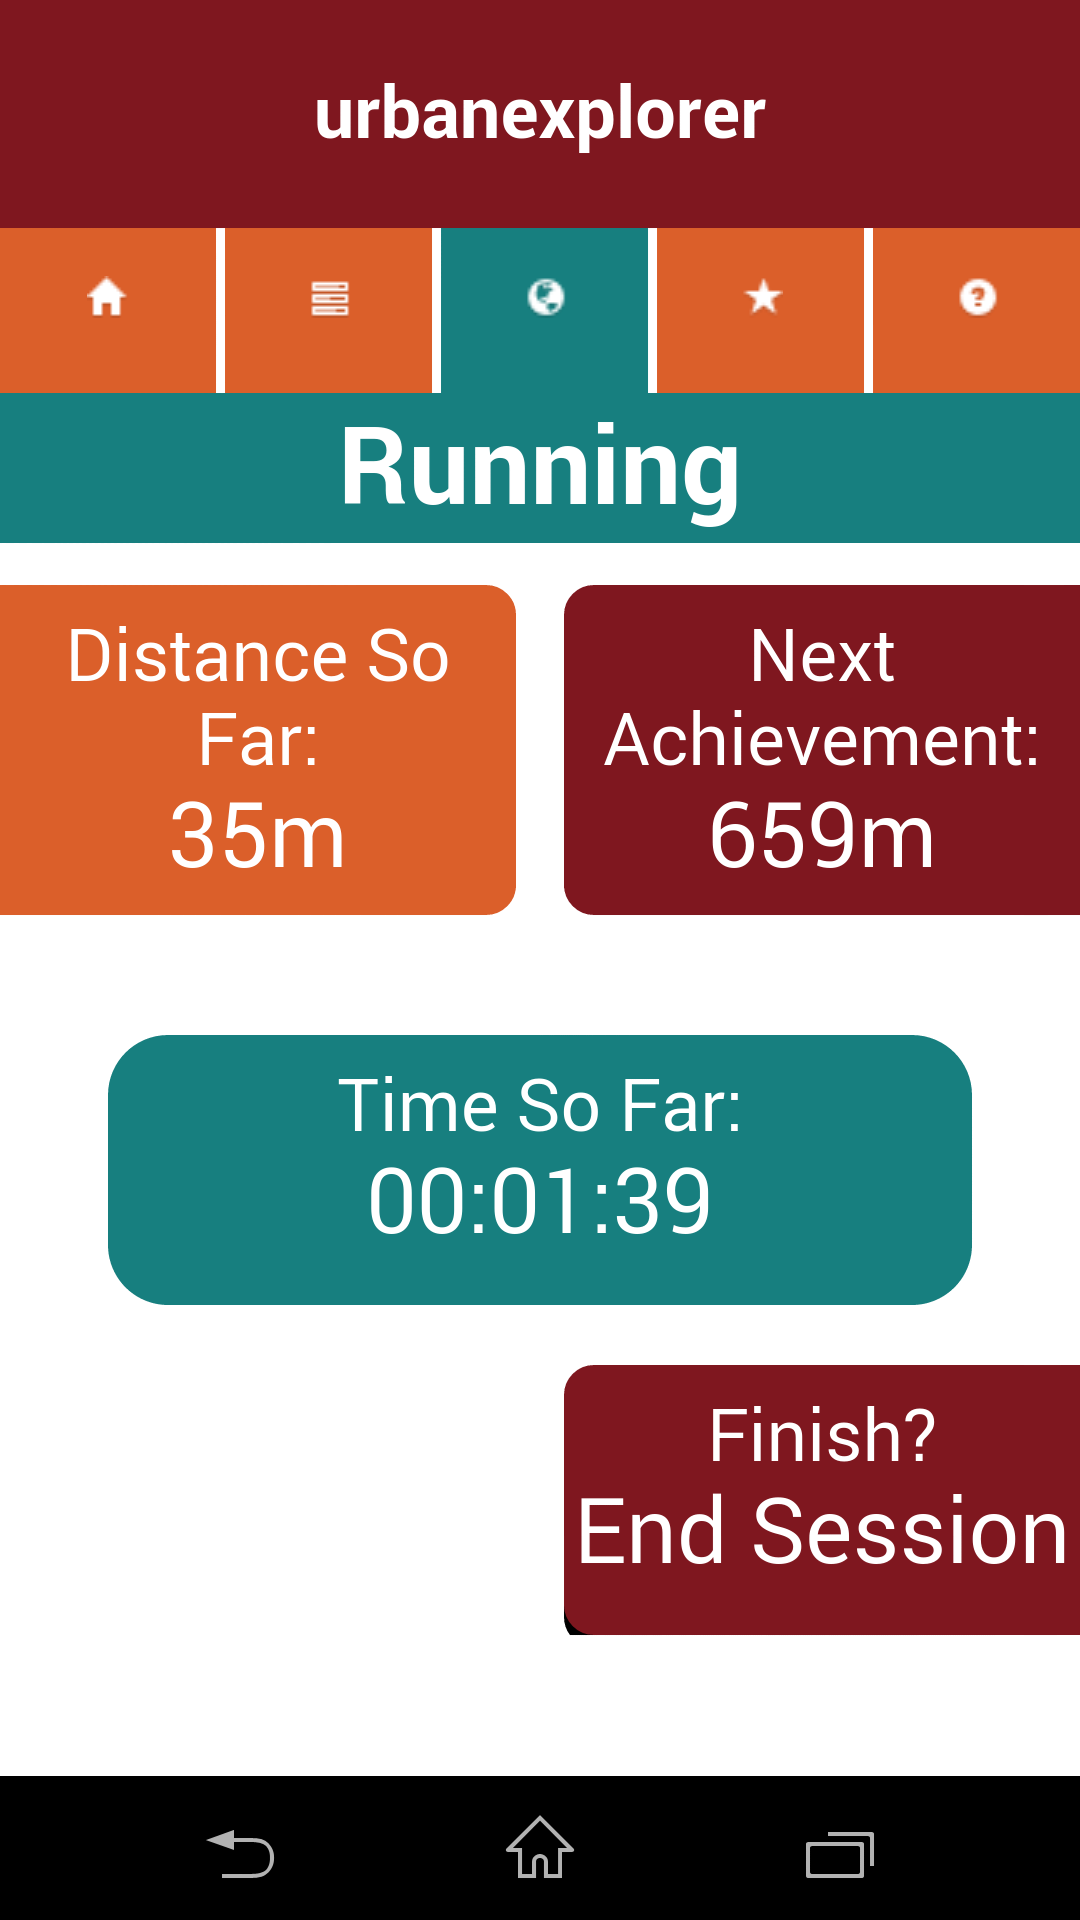
\includegraphics[width=0.29\textwidth]{images/init_design/run.png}
  \vspace{-20pt}
  \caption{Exercise Screen}
  \vspace{-25pt}
  \label{fig:init_run}
\end{wrapfigure}
When the initial design was formalised we did not have a solid idea of
what \emph{achievements} would be in the context of this
game. Therefore the concept of an \emph{achievement} does not feature
predominantly in this design iteration. 

Figure \ref{fig:init_run} shows the screen displayed when a user is
exercising. This screen is the key part of the application and was
given the most scrutiny. This design iteration had the same
functionality that the final design has in terms of the underlying
behaviour but users were quick to bring attention to the lack of
information displayed. The time and distance a user has travelled in
this exercise session (\emph{Distance So Far} and \emph{Time So Far})
and the distance until the next stage is completed (\emph{Next
  Achievement}) are displayed but there is no indication as to how far
along a route a user has progressed, or their overall time spent on
the route so far.  

It was recommended that by reducing the white space between elements
in the application we could easily include more information that was
relevant to the exercise session. One user indicated that a pictorial
representation of how far they had travelled along a route would be
desirable to see. The user likened the representation to a \emph{Horse
  Racing Derby
  Game}\footnote{\url{http://www.funfairstalls.co.uk/horse-racing-derby-game/4577291897}}
where the you have to complete a task, say rolling a ball into a hole,
and this advances your towards your goal, moving the horse closer to
the finish line. In our problem domain the task would be travelling
outdoors and the goal would be completing this route. By easily
substituting the horse model for a little running person we could map
our domain straight onto the fairground amusement. 

This idea was semi-realised in the final design and will be discussed
further in the final design section. It is important to note that a
user was able to comprehend the abstract nature of our gamification
goals and then interpret them in terms of a game they know and
understand. A key part of determining the validity of any form of
gamification is whether or not a user can understand what they need to
do to succeed. We discuss \emph{Routes} and \emph{Stages} in an
abstract sense as the user never physically travels along the path
that the \emph{Route} or \emph{Stage} defines, so it is rewarding to
discover that a user can make the connection between the abstract
depiction and a real world example.

Most users also commented on the colour scheme chosen for the first
design implementation. The garishness of the colours chosen was
apparent even before starting the first round of evaluation but
attention was drawn to what the colours can mean. Users commented that
using predominantly red colours may not be a good choice as the
application is intended to encourage, and red is not normally
associated with encouragement. An analysis by \citet{colours_red}
of how the colour red influences performance confirms this
speculation, however it is in a different problem domain. Future work
could be undertaken here to see if the findings of \citet{colours_red}
are consistent in an exercise domain. In our situation, the colour
scheme required attention so the decision was taken to respect the
literature and user feedback and change to a colour scheme that was
predominantly blue.

Users were asked what rewards they would want to receive as they
progress in this application to help influence our design
decisions. It was unanimously suggested that there should be a reward
for completing each \emph{Route} and most users suggested that this
reward should be time based. Not all users requested that a reward
should be given for completing a stages but this was formally added
after further discussion with the project supervisor. 

Attention was also drawn to a workflow subtlety which was causing
problems for users who had not enabled GPS before launching the
application. Normally this can be easily activated by opening the
task bar at the top of the screen but the app was designed to cover
this task bar so users had to find alternate ways to enable the GPS on
their device. The workaround the user was doing involved closing the
app entirely and then restarting it once GPS had been enabled. There
was no design justification to keep the task bar covered so the
app was changed to uncover it. Arguably the decision to uncover the
task bar is beneficial to the user in other ways as they can see other
notifications their device may give.

\begin{wrapfigure}{R}{0.29\textwidth}
  \vspace{-20pt}
  \centering
  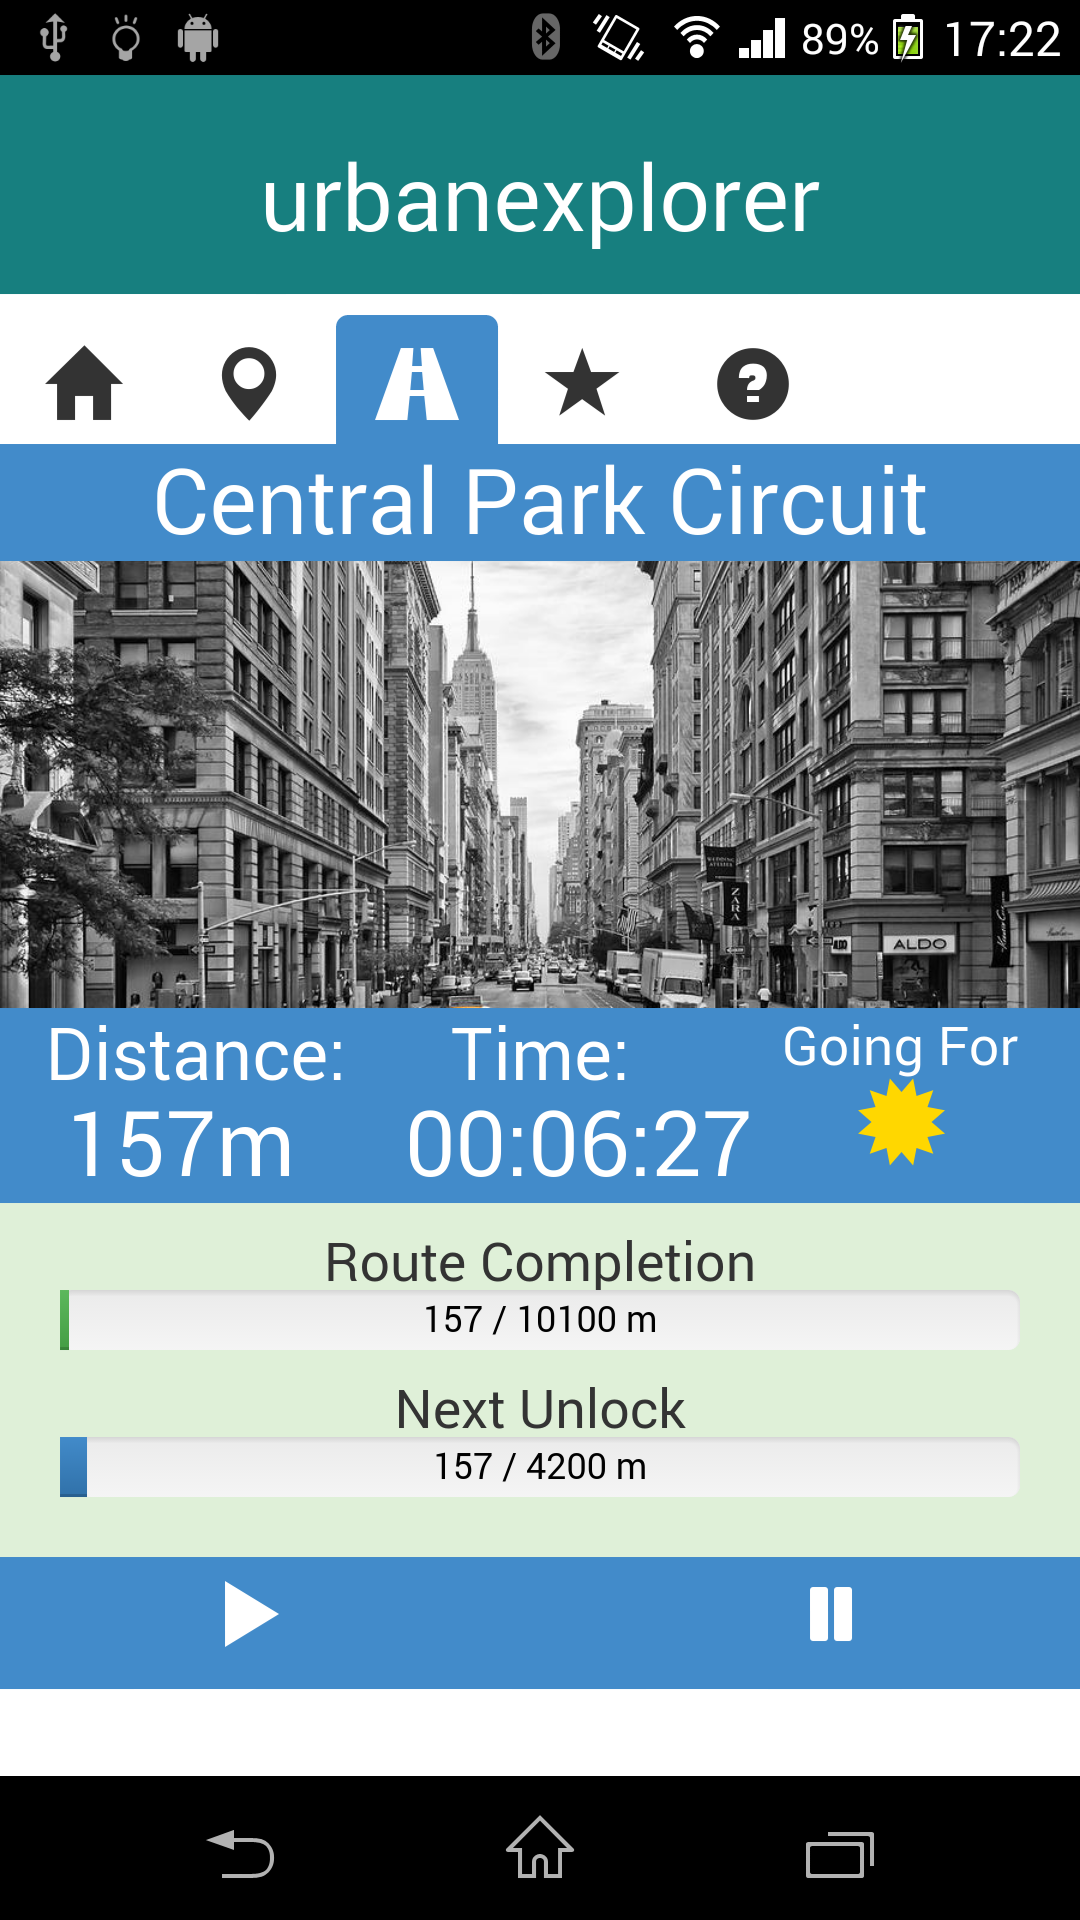
\includegraphics[width=0.29\textwidth]{images/screens/run.png}
  \vspace{-20pt}
  \caption{Exercise Screen}
  \vspace{-35pt}
  \label{fig:final_run}
\end{wrapfigure}

With feedback from the first iteration of design, the final design was
implemented. This was distributed to a larger group than the first
design iteration and feedback was received largely through word of mouth
and also through an online survey.

The changes made to the screen shown when a user is exercising can be
seen in Figure \ref{fig:final_run}. In this final design, the Twitter
Bootstrap\cite{bootstrap} CSS framework was used as the main
structural backbone of the app layout. This provided better support
for small screen devices and convenient features such as a colour
palette complementary to the colours we desire and a large set of
ready-made navigation icons.

The \emph{achievement} structure was formalised after the first design
iteration so we endeavoured to include these in the most appropriate
ways in the final design. The picture you unlock by completing the
\emph{stage} you are currently on is now a featured part of this
screen. Predominance was given to this element as it is very visually
appealing and it also enhances the \emph{story} of the game (as
discussed in Section \ref{sec:gamification}). We want the user to
engage in the \emph{story} we are creating, so by explicitly showing
the user a graphical representation of the abstract \emph{route} they
are travelling along they are invited to believe that they are running
near the area set by the abstract \emph{route} and not the area they
are physically in. 

There is little unused screen space in this design iteration and this
was met with positive feedback from users. We should note that not all
information was able to be presented to the user: the overall time
that a user has spent on a \emph{route} is not shown here. This was
due to a suitable layout not being discovered during the final design
phase and future work should be dedicated to further revising this. 

\begin{wrapfigure}{R}{0.29\textwidth}
  \vspace{-20pt}
  \centering
  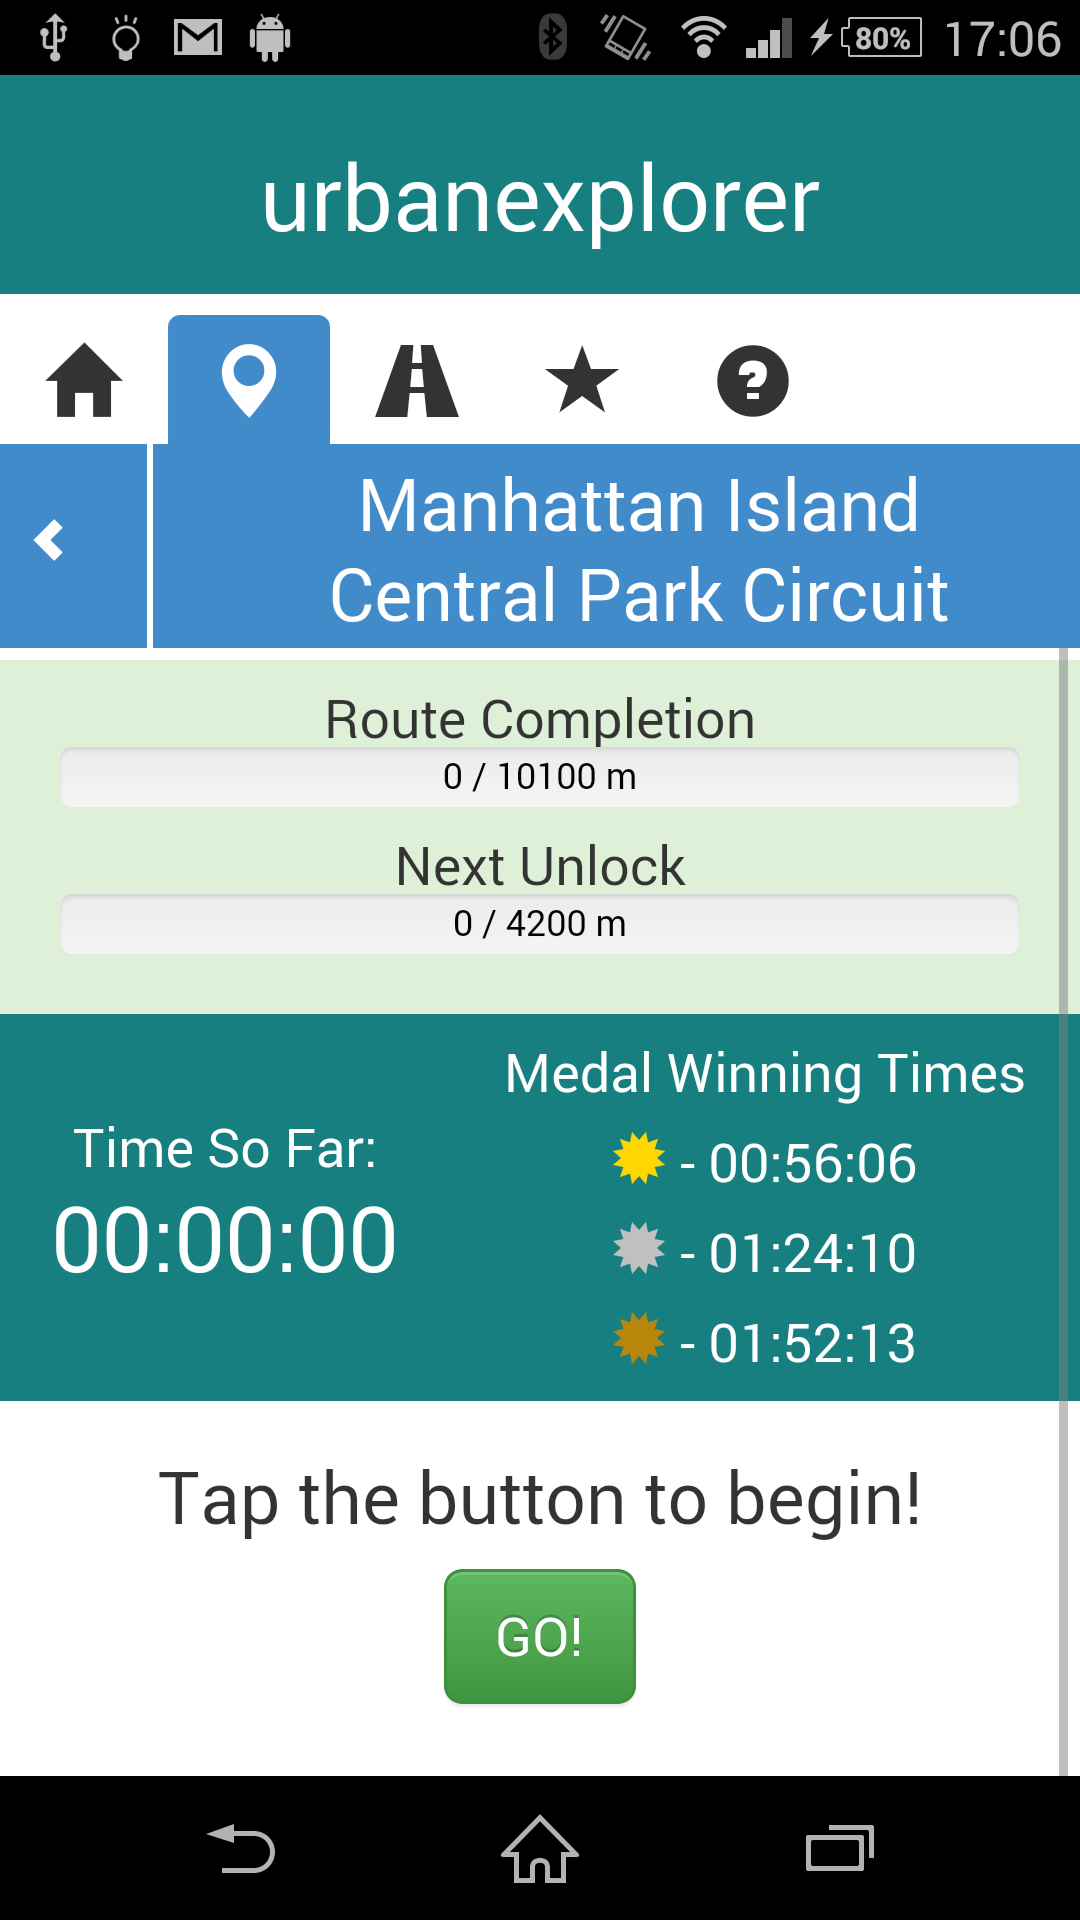
\includegraphics[width=0.29\textwidth]{images/screens/route.png}
  \vspace{-20pt}
  \caption{Route Info Screen}
  \vspace{-65pt}
  \label{fig:final_route}
\end{wrapfigure}

We have also included in Figure \ref{fig:final_run} an indicator as to
the best medal a user could achieve given their current time on a
\emph{route}. Combined with the screen depicted in Figure
\ref{fig:final_route}(the screen that a user is shown after they have 
picked a \emph{route} to travel on which shows the user how much time
they have on a \emph{route} before they exercise) the problem is
alleviated but the issue is not fixed completely. Figure
\ref{fig:final_run} also shows the \emph{``Medal Winning Times''}
for this \emph{route}.

The way that progress is shown in final design iteration differs
greatly from the initial design. Effort was made to include the
metaphor of the \emph{Horse Racing Derby Game} progress visualisation
in the final design. Although there is no explicit graphical
representation of a person running, this progress visualisation can be
seen through the two bars marked \emph{Route Completion} and
\emph{Next Unlock}. These bars fill from left to right as the user
progresses along a route towards completion. Feedback from users was
positive about this change, noting that it was much easier to glance
at the screen to see how close you were to achieving a goal when you
were exercising and that it was satisfying to look back at your
progress along routes when you are browsing which route you want to
travel along. 

\begin{wrapfigure}{R}{0.29\textwidth}
  \vspace{15pt}
  \centering
  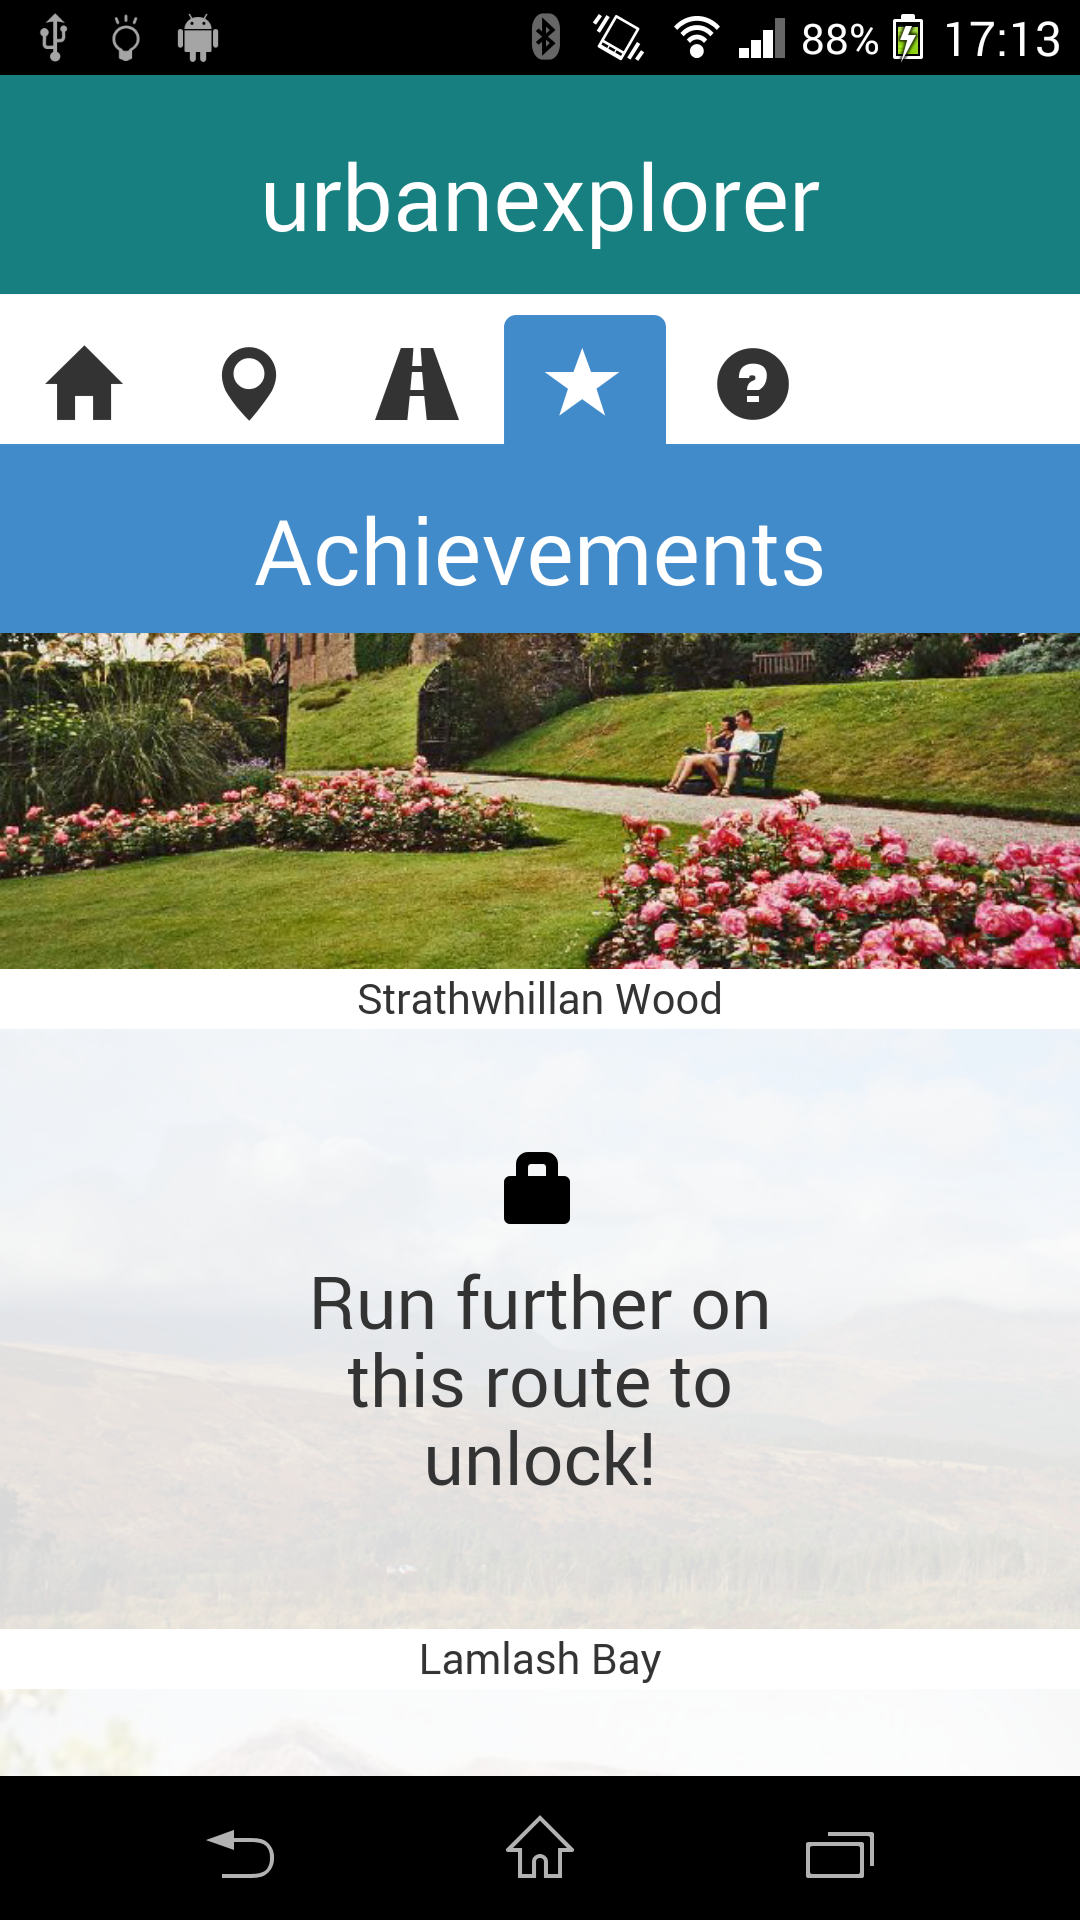
\includegraphics[width=0.29\textwidth]{images/screens/ach_2.png}
  \vspace{-20pt}
  \caption{Achievement Screen}
  \vspace{-25pt}
  \label{fig:final_ach}
\end{wrapfigure}

No explicit comments were given regarding the change in colour scheme
although users did compliment that the style was ``pleasing'', a great
improvement on the previous criticism. 

The achievements screen displayed in Figure \ref{fig:final_ach} also
received little explicit feedback. In this screen the unlocked
pictures are displayed for a user to peruse at their leisure. At no
point during the exercise workflow is the user directed towards this
section so discovery of this page is only achieved through exploration
of the app. This workflow design flaw may be the root cause of little
feedback for this section and future work should make this section
more predominant. The logical place to direct a user to this section
would be after a user completes an exercise session as it is at this
time that new pictures are likely to be unlocked. 

A breaking problem that persisted from the first design iteration to
the final design concerns the middle tab in the navigation bar: the
exercise tab. This tab is only active when a user is exercising and at
all other times will redirect the user to the route selection screen
(selected by the second tab from the left) if the user should click
it. This was created with the best intentions of correcting a users
behaviour: an exercise session can only start if the user has selected
a route to travel along and so seems logical to direct the user here
to select one. However this caused confusion with users as they
believed that, since they could not select the tab, it was broken
entirely. A redesign of this top-level navigation is therefore
required to remove this confusion.

\subsection{Future Design Work}
The final design of this project requires work to become a design
worthy of a marketable product. Future work suggested by the author
and some features requested by users are as follows:

\begin{itemize}
  \item An indicator inside the app that lets the user know whether or
    not their GPS is turned on or not. This indicator should also
    allow the user to turn on GPS if it is not activated.
  \item An indication in the task
    bar\footnote{\url{http://developer.android.com/guide/topics/ui/notifiers/notifications.html}}
    that the app is running (one user said they forgot it was on and
    the GPS drained the battery). This indication could also show the
    progress through a bar in a similar way to how it is shown in the
    exercise screen (Figure \ref{fig:final_run}).
  \item Redesign the top-level navigation bar to make navigation more
    intuitive. 
  \item A full analysis of colour as an encouragement factor. As was
    discussed previously, some literature argues that predominantly
    red colour schemes reduces performance\cite{colours_red} but red
    can also be associated with a feeling of power. An analysis should
    be done to see if colours are perceived in an exercise context in
    the same way as a non-exercise context, the result of which would
    be used to influence the colour palette in the application.
  \item A larger predominance of the \emph{stage} completion
    achievements is required to enforce short-term success. More
    emphasis should be given on rewarding the user  when they unlock a
    picture. 
  \item More emphasis should be given in general when a user achieves
    something. Currently there is no visible or haptic notification
    that the user has actually achieved something as it
    happens. Future work should aim to add some form of notification
    at a bare minimum.
\end{itemize}

\section{Evaluation of Gamification}
\subsection{Comments From Evaluation}
A quantifiable measure of the effectiveness of gamification in this
project would likely be unsubstantiated due to the short duration of 
the experiment. Since we are unable to observe the long-term progress
of a user engaging with this platform, we are unable to identify
trends in behaviour that could indicate behavioural change. However we
can speculate how the platform may progress based on feedback from
users and propose what additions to the gamification experience may be
necessary to improve the chance of success.

By the end of the evaluation the app had been downloaded 39  times and
9 users had engaged in the gamified experience. Of these users who
had engaged with the gamified experience, three had unlocked pictures
by completing stages and two received a medal (a \emph{gold} and a
\emph{silver}). Engagement was tracked through time spent exercising
and we state that a user has engaged if we have any logged time of
that user exercising. The results of those users who engaged with
the app are shown in Table \ref{table:usage}.

\begin{table}[h]
  \centering
  \begin{tabular}{| c | c | c | c | c | c | c |} \hline
    % Headings
    ID & 
    \multicolumn{1}{p{1.7cm}|}{\centering Total Time \\ (hh:mm:ss)} & 
    \multicolumn{1}{p{2.1cm}|}{\centering Distance \\ Travelled (m)} &
    \multicolumn{1}{p{1.7cm}|}{\centering Stages \\ Completed} & 
    \multicolumn{1}{p{1.7cm}|}{\centering Routes \\ Completed} &
    \multicolumn{1}{p{1.5cm}|}{\centering Exercise \\ Sessions} &
    Medals Won \\\hline
    %% Content
    e4ade9027f33ceee & 09:40:46 & 20027 & 11 & 4 & 1 & - \\\hline
    9484f35fe45a0870 & 03:17:51 & 11805 & 5 & 1 & 2 & 1 $\times$ Silver \\\hline
    5e029a949fdfad8f & 02:16:10 & 4038 & 0 & 0 & 1 & - \\\hline
    2a46006a774cd542 & 01:54:42 & 15141 & 39 & 2 & 3 & 1 $\times$ Gold \\\hline
    56a8db4c54d600b4 & 00:02:02 & 2 & 0 & 0 & 2 & - \\\hline
    7ee212a0e8319b69 & 00:01:21 & 74 & 0 & 0 & 2 & - \\\hline
    d3ff351879e910ba & 00:01:10 & 103 & 0 & 0 & 1 & - \\\hline
    367542602d7d9cda & 00:00:20 & 23 & 0 & 0 & 2 & - \\\hline
    465ca59228c4f805 & 00:00:01 & 0 & 0 & 0 & 1 & - \\\hline
  \end{tabular}
  \caption{Active users of ``Urban Explorer'' ranked by time invested.}
  \label{table:usage}
\end{table}

A survey was given to users where they were asked to indicate how
encouraging they perceived each part of the application to be. The
survey received eight responses which generally align with the
empirical data we gathered. A summary of the responses are as follows:

\begin{itemize}
  \item Seven out of eight responses state that, on average, they
    exercise less than three hours a week and four responses state
    that it is less than one hour a week; but only four responses overall
    state that this exercise occurs outdoors. Two responses state that
    this exercise occurs in a gym and five users state that they
    exercise in their own home (note that users could pick multiple
    locations where they exercise). 
  \item There was an equal split in responses with those who have used
    technology before in exercise and those who had not; but only two
    responses state they have formally tracked their exercise
    previously. 
  \item The majority of responses stated that they used the app
    between one and three times, which aligns with the empirical data
    in Table \ref{table:usage}.
  \item Responses indicate a positive experience with the app. From a
    five-point rating scale, responses gave navigation a 3.88 score and
    route selection a 4.5 score. Goal awareness for what was required
    to receive a medal was given a 4.13 score and unlocking a picture
    was given a 3.38 score.
  \item On a five-point rating scale, completing routes to obtain
    medals was scored highest in terms of encouragement, scoring 4.14,
    and unlocking pictures scored lowest, scoring 3.43. Viewing
    pictures of the route you are on as you are exercising was met
    with a better response (scoring 3.57) and showing absolute statistics
    about your exercise was also liked (scoring 3.71).
  \item From a five-point rating scale, responses indicated a
    dissatisfaction with how often the app updated the distance
    (scoring 2.83 from 6 responses). Responses were divided over
    whether or not the app reported distance accurately (scoring 3
    exactly). 
  \item The goals in the app were very clear to those who
    responded. On a five-point rating scale the clarity of the goals
    scored 4.33 and the encouragement of the goals scored 3.5.
\end{itemize}

Responses indicated a generally positive experience with the app and
the game concepts implemented. Since the majority of responses
indicate that they do not meet the current exercise guidelines of
between 75 and 150 minutes of exercise, as defined in the Health Survey
for England \cite{exercise_2012}, we have received responses from our
targeted user group. 

The long-term goal reward of being awarded a \emph{medal} for
completing a \emph{route} was met with good feedback, but it is
unfortunate to note that the rewards for short-term goals were not as
well received (being ranked lower in terms of effectiveness than
statistics alone). This could be in part to an overall lack of
exposure to the short-term rewards in the exercise work
flow. Short-term goals are essential to keeping a user motivated so
that they can achieve the more rewarding long-term goals. A different
kind of reward entirely may be more appropriate but work should
certainly be undertaken to determine why this encouragement is not as
effective. 

An improvement is also required to make the user trust the distance
reported by the app. The way that the user plays the game is by
travelling outside and if the user cannot engage with the progress
feedback that is provided because it is either not frequent enough or
is not accurate then this creates a pertinent cause for concern. A
user has no reason to engage in a game if they do not believe that the
actions they make influence their success in the game. By dealing with
the \emph{Cul-de-sac} effect (Section \ref{sec:location_mgmt}) we can
improve confidence in the user that the distance the app thinks the
user has travelled is correct. 

From the nine users who engaged with the gamified experience (Table
\ref{table:usage}) only four of these users actively used the
application, based on the total time and distance travelled of these
nine users. These users invested a significant amount of time in the
application which indicates they enjoyed their experience with
``Urban Explorer''. The top row in the table states that one user
exercised for almost ten hours, continuously, in one exercise session
and travelled over 20km. It is very unlikely that the user was
explicitly exercising for this time duration and more likely left the
app running in the background while going about their daily routine,
possibly travelling by car or bus, having forgotten to turn it
off. 

A previously unconsidered use case of this app would be to do
exactly as we propose this user has done, leaving the app open in
the background as they went about their daily routine. Since our
rewards are temporally based, users are disadvantaged by having the
app running in an exercise session and not actually moving. We could
detect when a user is not moving and stop accumulating time and
distance and then reactivate this tracking when they do start moving
again. This would be interesting future work as users may wish to
interact with the app in a less direct way, similar to the interaction
with the Fitbit devices (Section \ref{sec:fitbit}).

Since overall interactions were low in comparison to overall downloads,
of which there were 39 downloads compared with three or four full
engagements, a better \emph{onboarding} strategy should be implemented
to familiarise users with the game aspects of the
app. \emph{Onboarding} is the process of introducing users to a
particular process where the user can both interact with the process
and control the outcome with positive benefits to the user. Currently
the \emph{onboarding} process in ``Urban Explorer'' is very minimal
with an explanation of the goals and exercise process only found in
the help section. We rely on the user exploring the application to
discover how to start an exercise session and so better direction 
could be given to encourage users to start engaging with the app
fully. 

Overall, feedback from users about the game experience was generally
positive with users engaging with the concepts required for achieving
long-term goals. 

\subsection{Future Gamification Work}
The core game ideas included in this project indicate that users could
be encouraged to exercise in the way we propose. The concepts explored
in this project are a small part of what could be used to encourage
users. 

One user commented:
\begin{quote}
  I don't feel as motivated as I might have done; notifications
  reminding me to walk would have been of great benefit. I wish it
  synced with my Google Calender so I could see how far I had walked
  and when. 
\end{quote}
Both of these comments are perfectly reasonable suggestions and would
be recommended as potential avenues for expansion. The first
suggestion is not specifically gamification but is a reminder to the
user to play the game. After a user has used the app for a reasonable
time period we could identify when a user is likely to exercise next
and send an encouraging notification to the user to reinforce their
exercise schedule. This encouragement could be based on their current
exercise status (``You're really close to finishing the Central Park
Circuit! If you run like you did on Tuesday you'll easily get it!'')
or purely based on user statistics (``You almost ran further yesterday
than you ever did before, think you can beat it today?''). 

Syncing with a calender, or simply allowing a user to track their
exercise history is more gamified and would be a valuable addition to
the system. We can praise the user for their progress but self
discovery of their trends will be rewarding for the user, helping them
better understand their exercise development. We could present this to
the user on a leaderboard where their exercise sessions are ranked
based on their personal performance. A social element could be
integrated here where they can compare their performance with other
users. Competition between users is a good way to encourage better
performance per user, but we should be careful that it does not become
discouraging to slower users or those users who are performing well
but are incomparable to the best users. Exactly how to manage this
situation is not clear, but splitting the leaderboards in a
hierarchical way based on region may be a good place to start. In this
situation your performance is only compared with your local peers
until you reach the top of the leaderboard in your area when your
performance would then be compared with peers at the top of other
leaderboards in other areas. 

Collaboration between users would also be an effective encouragement
tool. Socially you could create a team of peers in your local area
where your accumulated distance between all peers contributed towards
the progress of much longer routes, John O'Groats  to Land's End for
example. Alternatively the real-world social element could be removed
altogether and exponentially larger routes could be completed with all
users in the game, where collectively the users could contribute to a
``Run Around The World''. It would be important in either of these
cases to ensure that users did not ride on other users successes, that
is to say that all peers in a team would need to contribute a
certain distance each for the award to be valid. This is an issue that
could be explored more fully in the future, however.

The canonical sharing exercise session results and awards to social
networking sites or amongst peers could encourage users but this may
not be enough to actually motivate users to exercise and solve our
original \emph{problem}. It could help to breach the initial topic of
social exercise amongst a users peer group in a similar way to how
\emph{Chick Clique} (Section \ref{sec:gamification}) helped the girls
approach the discussion of healthy eating, but it would most likely
not be enough to be a proper encouragement technique. 

A change to the way the game is formed could also increase motivation
by adding a discovery aspect to the game. When discussing the Entity
Relation diagram in Section \ref{sec:ER}, the idea of representing
\emph{routes} on a map was introduced. In this approach a user would
start at one \emph{place} such as Glasgow and travel along a
\emph{route} to Edinburgh which would in turn unlock \emph{routes} to
other \emph{places} that can only be reached from Edinburgh. This
introduces a \emph{discovery} element to the game where a user must
travel between \emph{places} to discover new content. Consistency
would not necessarily be enforced here: we could allow a user to
travel from Glasgow to Edinburgh, which logically would put the user
in Edinburgh in the game, but we could immediately allow the user to
travel another \emph{route} leaving Glasgow to accommodate for faster
game progression.

With this new concept we could also introduce an in-game passport
where the user receives a stamp in the passport for every location
they have travelled to. We can then create even longer-term goals
where a user would receive a big reward for reaching every
\emph{place} in a geographical area, the major cities in Scotland for
example. For users who have invested considerable time in the story of
the app, this may prove to be very encouraging as it gives them harder
to achieve goals that can be achieved without changing their current
behaviour. 

The proposed future work here is mainly speculative based on feedback
from users and the thoughts of the author. A longer experiment would
yield more conclusive results about how effective the current
gamification methods are, which in turn may create a better founding
for the proposed future work, but there is certainly room for
expanding the gamified experience in ``Urban Explorer''.


\section{Evaluation of Platform}
PhoneGap has its merits as a mobile platform: you can achieve rapid
development cycles by taking advantage of strong JavaScript and CSS
frameworks, a ``write once, deploy anywhere'' strategy for multiple
platform development, and good integration with the phones native
functionality. However it is the details of the integration with the
native functionality that can leave wanting, especially for
geolocation information.

As is discussed in Section \ref{sec:location_mgmt}, we use the PhoneGap
provided location watch service to receive location information. It
was discovered during development that if the PhoneGap provided
location watch service could not obtain location information for any
reason then the request would fail silently. Geolocation information
cannot always be obtained due to factors outwith our control and so
failing silently does not allow the developer to enforce any form of
control when searching for location information. We have discussed in
Section \ref{sec:location_mgmt} how we can manage the location
information, but if we make a request to the framework to provide us
with location information then it is pertinent that either we receive
this information or we are notified that this information cannot be
obtained. By failing silently the programmer has no way of handling
the situation and so users were left in a state of confusion as to
what the app was doing. This is a major issue in the scope of this
project due to the heavy reliance on location information and until it
is fixed it could not be reliably used in a production environment. 

Other small issues that prevent a recommendation that PhoneGap is a 
production quality framework include: a provided build script to build
a ``release'' version of the app for the Android Play Store builds a
``debug'' version instead, each time you build the app the version
number and release number are reset to their default values, a
configuration file for the app is ignored when searching for the main
``index.html'' file (root of the application), and the official
documentation does not agree internally\cite{phonegap_install,
  phonegap_cli, phonegap_geolocationAccessingFeature}.

However, as a platform that allows you to prototype ideas and designs,
it is ideal as you can rapidly prototype for multiple devices without
needing explicit knowledge of the actual domain (you do not need to
know specifics about programming for Android or iOS). It is unlikely
that the two design revisions would have been achieved as completely
as they were in this project if PhoneGap was not used. It is worth
noting that no user noticed that the app was not created as a native
Android app.

The author would recommend that for this product to be marketable, it
should be implemented as a native Android application. By doing this
greater control is obtained over the location information,
specifically through the Google Play Location
Services\footnote{\url{https://developer.android.com/google/play-services/location.html}}
which have better management of power and accuracy than other
techniques. Rapid prototyping of ideas could still be undertaken using
PhoneGap but a more refined app would be produced by a native Android
implementation. There is the downside that explicit platform knowledge
is now required to produce the app, especially for multi-platform
development (Android and iOS) but access to better control over the
location services outweighs this issue. 

From the server perspective, the author sees no reason to move from
the Django middleware service and the Django-Tastypie based API. No
issues have arisen from the use of either part of the system, both
fulfilling the requirements of the entire system very well. 
